\section{问题二的模型建立与求解}

问题二从共同初值 $T(r,0)=301.15\,\mathrm K$、$C(r,0)=2.55$ 重新开始，全程采用附录 3 的变物性关系：$\rho,c_p,k$ 随 $C$ 变化，$D(T,C)$ 同时受温度和含水率影响。已有耦合干燥研究采用联合热质传递模型描述状态依赖扩散率[\cite{ref5}]。控制方程仍为
\[
 \rho(C)c_p(C)T_t=\frac1r\partial_r(rk(C)T_r),\qquad C_t=\frac1r\partial_r(rD(T,C)C_r),
\]
但两场通过物性形成双向反馈，必须联合推进。水分通量只对含水率因子作 Kirchhoff 积分，温度因子保留在界面系数中；表面半控制体仍通过 Robin 方程求解真实表面状态。

正式网格为 $N=1024$，采用相对容差 $2\times10^{-7}$、绝对容差 $2\times10^{-9}$ 和最大步长 $300\,\mathrm s$。
\begin{table}[H]\centering\small\caption{问题二 3 h 内药材温度（$^\circ$C）}\label{tab:q2temp}\resizebox{\textwidth}{!}{\begin{tabular}{rrrrrr}\toprule 时间/h&0 cm&0.5 cm&1 cm&1.5 cm&2 cm\\\midrule 0.5&32.1893&32.3821&32.9660&33.9608&35.4130\\1.0&40.3815&40.5535&41.0605&41.8782&42.9976\\1.5&45.8465&45.9346&46.1928&46.6049&47.1399\\2.0&48.4496&48.4875&48.5979&48.7730&49.0029\\2.5&49.4667&49.4789&49.5133&49.5650&49.6607\\3.0&49.8494&49.8552&49.8744&49.9100&49.9663\\\bottomrule\end{tabular}}\end{table}
\begin{table}[H]\centering\small\caption{问题二 3 h 内药材含水率（kg/kg）}\label{tab:q2moisture}\resizebox{\textwidth}{!}{\begin{tabular}{rrrrrr}\toprule 时间/h&0 cm&0.5 cm&1 cm&1.5 cm&2 cm\\\midrule 0.5&2.5499&2.5489&2.5256&2.3257&1.6486\\1.0&2.5257&2.4948&2.3578&2.0230&1.4711\\1.5&2.3861&2.3256&2.1344&1.8020&1.3476\\2.0&2.1709&2.1084&1.9236&1.6259&1.2311\\2.5&1.9567&1.9006&1.7360&1.4720&1.1167\\3.0&1.7662&1.7165&1.5702&1.3333&1.0081\\\bottomrule\end{tabular}}\end{table}
表 3 和表 4 的原始数据见 \texttt{results/q2/table3.csv} 和 \texttt{results/q2/table4.csv}。

\begin{figure}[H]
  \centering
  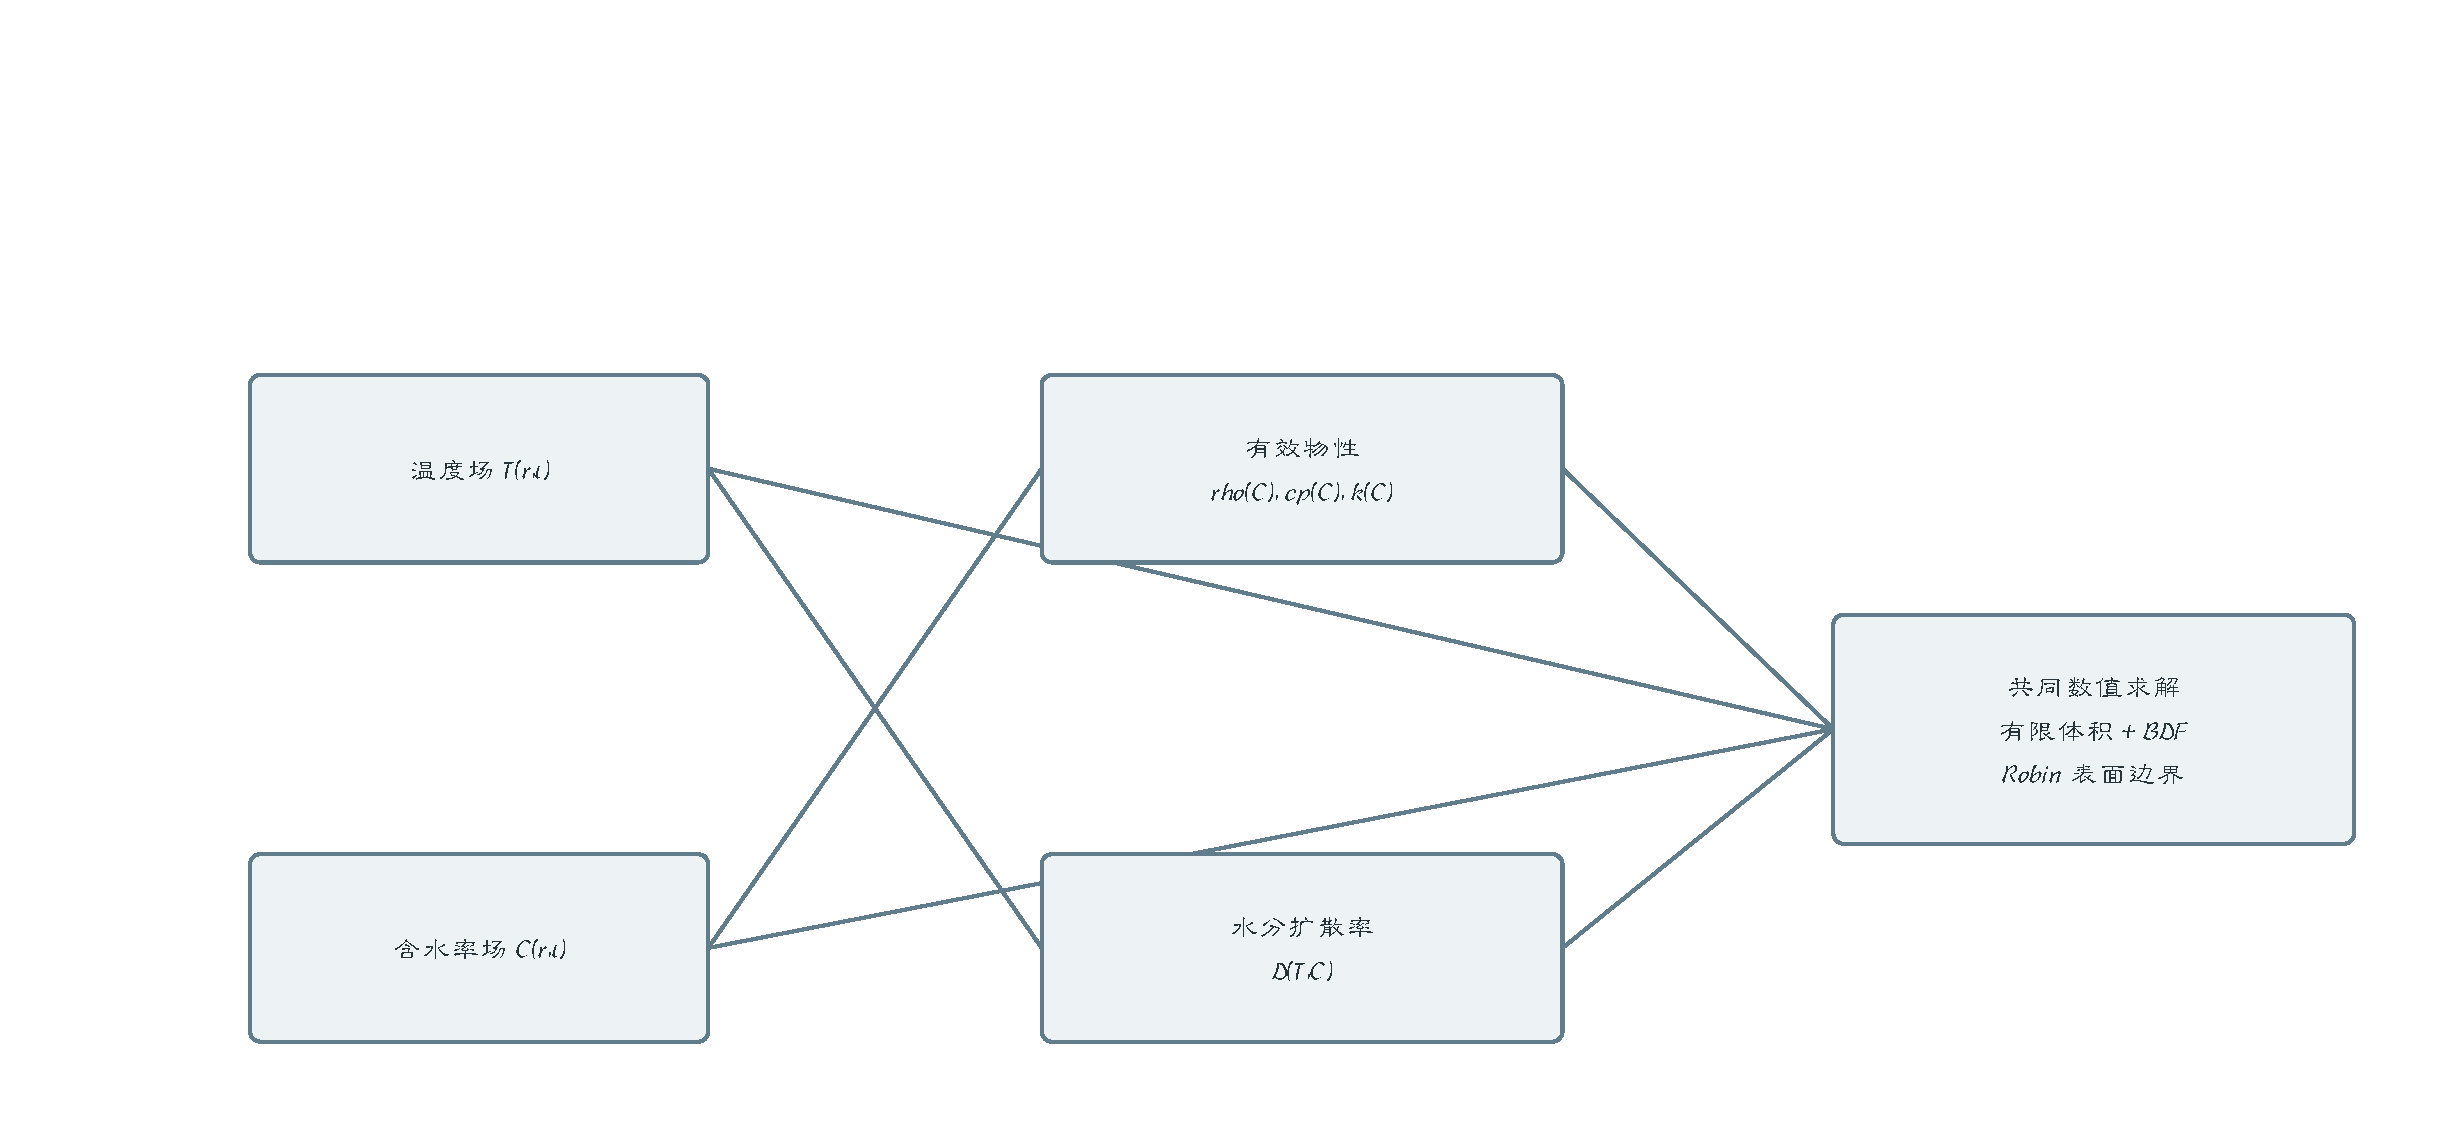
\includegraphics[width=0.78\textwidth]{../figures/q2/fig_q2_coupling.pdf}
  \caption{问题二温度—含水率物性反馈结构}
  \label{fig:q2coupling}
\end{figure}

图~\ref{fig:q2coupling}概括变物性反馈关系；温度场在 3 h 内逐渐接近环境，含水率变化主要从表层向中心传播。网格由 1024 加密至 2048 时，最大温度和含水率差分别为 $1.163\times10^{-6}\,\mathrm K$ 和 $4.243\times10^{-7}\,\mathrm{kg/kg}$；收紧时间设置后的差异分别为 $5.912\times10^{-4}\,\mathrm K$ 和 $1.429\times10^{-5}\,\mathrm{kg/kg}$。干基水量收支残差为 $2.665\times10^{-15}$。
